\chapter{The First Series (1999)}
\label{c:first-series}
%\newcounter{foot}

The ideas and results that have been discussed in Part I of the present volume 
were based on results obtained in idealised conditions. Computer simulations are able to 
test the validity of the basic algorithms, but simulations are still theoretical in nature. 
It is well known that technologies can only become a reality after 
experiments have been carried out in open-ended real world conditions. Nobody would want to fly an airplane that 
has only been tested in computer simulations. 

We did the same for the Talking heads experiments and this was a huge step. Many more people had to get
get involved: for making the code more robust, setting up the teleportation infrastructure, and installing and 
maintaining the physical installations in different countries.  
The mechanisms about language evolution discussed in Part I of this book did not significantly change. On the contrary, 
they received solid experimental confirmation. At the same time, we learned a huge amount about the dependencies
between these mechanisms and the environments in which agents use them. We also learned a great deal about running software 
agents in an open infrastructure distributed over the entire globe. Furthermore we learned a lot 
about the interaction between humans and agents ranging from 
enthusiastic participation and enjoyment to nasty attacks by English hackers, set on destroying the experiment. 

This chapter provides more detail on the first main experiment that took place in the summer of 1999 as 
part of the Laboratorium exhibition in Antwerp. The next chapter documents follow up experiments that took place
within the context of the N01SE exhibition in Cambridge and London and at several other locations. 

\section{The Laboratorum Exhibition} 

The Laboratorium\is{Laboratorium exhibition}
exhibition was a major artistic event in Europe during the summer of 1999 organised by 
Bruno Verbergt of an organisation called 'Antwerpen Open'.
It was one of the first exhibitions that put so much emphasis on art as a research 
activity and on profound interactions between art and science.
Participants included both scientists and science historians such as Peter Galison, Bruno Latour, Israel Rosenfield
and Isabelle Stengers, as well as architects such as Rem Koolhaas and artists with an affinity for research 
such as Peter Fischli and David Weiss, Gabriel Orozco, Carsten H\"oller, Panamarenko, Lawrence Weiner a.o. 
The exhibition was visited by 8000 people. 

The introduction to the catalog edited by curators Hans Ulrich Obrist
and Barbara Vanderlinden\footnote{
The catalog of the Laboratorium exhibition was published as 
\cite{Obrist:1999}.} stated the objectives as follows: 
\begin{quotation}
{ Laboratorium is an interdisciplinary project in which the scientific laboratory and the artist's studio are explored
on the basis of their various concepts within the different disciplines. How can we attempt to bridge the gap between 
the specialized vocabulary of science, art and the general interest of the audience, between the expertise of skilled
practitioners and the concerns and preconcepts of the interested audience? 

Laboratorium will search the limits and possibilities of the places where knowledge and culture are made. Throughout 
the summer we will establish within the city of Antwerpen networks, fluctuating between highly specialized work by 
scientists, artists, dancers, and writers. "Working places" where the participants communicate their findings on the 
"work in progress". Also the scientific laboratories in Antwerpen will be involved in the initiative. 

Laboratorium started as a discussion that involves questions such as: What is the meaning of laboratories? What is 
the meaning of experiments? When do experiments become public and when does the result of an experiment reach 
public consensus? Is rendering public what happens inside the laboratory of the scientist and the studio of the 
artist a contradiction in terms? These and other questions are being offered in this interdisciplinary project 
that starts with the "workplace" where the artists and the scientists experiment and work freely.}
\end{quotation}

The event was part of the activities, celebrating the famous Antwerp painter Anthony van Dyck born 400 years earlier.
In preparation of the exhibition a series of discussions were held between  
Carsten H\"{o}ller, Bruno Latour, Hans-Ulrich Obrist, Luc Steels and Barbara Vanderlinden. These discussions helped 
to shape the general concept of the exhibition and the selection of the artists and scientists who would participate. 
Excerpts appeared in the exhibition catalog and other publication fora, \cite{Obrist:2003}. 

The exhibition took place in two locations: the photography museum in Antwerp, which was the main location, and an annex 
occupying several floors in a high rise office building close to the central station (the so called President's
Building). The Photography Museum Exhibition featured work by several well known artists, architects and scientists. 
The annex featured the Talking Heads experiment as well as 
work by artists Joseph Grigely and Matt Mullican and science philosopher 
Isabelle Stengers, who had set up a reconstruction of Galileo's famous experiments. 
There were also a number of public presentations under the heading 
"The Theatre of Proof", organised by Bruno Latour. The catalog was designed by Bruce Mau and his team. 

\begin{figure}[htbp]
  \centerline{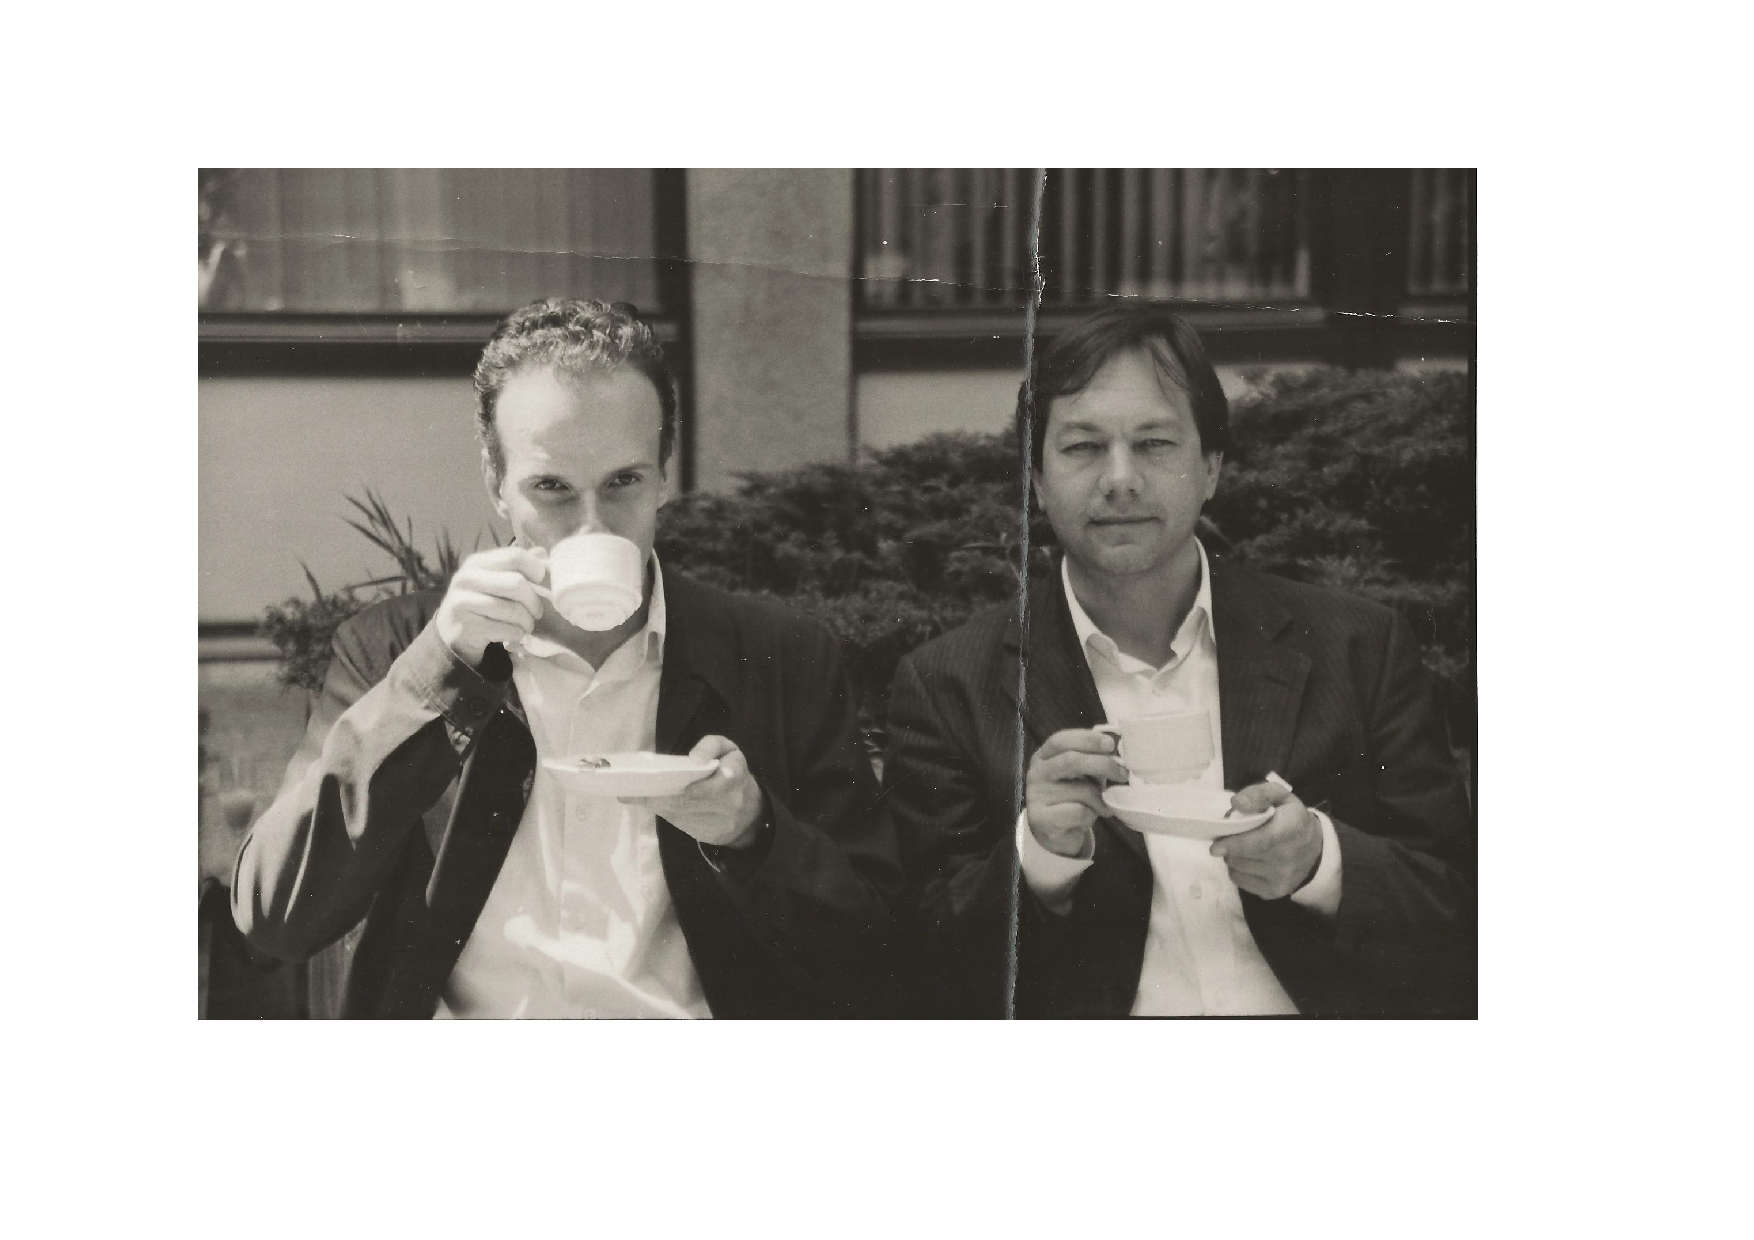
\includegraphics[width=0.7\textwidth]{chap8/figures/hu-obrist+ls}}
\caption{ \label{fig:faces} 
Hans-Ulrich Obrist and Luc Steels during the opening of the Laboratorium Exhibition in Antwerp, summer 1999. }
\end{figure}
In addition to the installation at the exhibition in Antwerp itself, there were two additional 
external sites for the Talking Heads experiment operating within the same time frame: The Paris site at the Sony Computer 
Science Laboratory in Paris and the Brussels site at the Free University (Vrije Universiteit) of Brussels.

Months of preparation and testing took place before we attempted to go 'live' and public. 
Once this happened, work continued frantically to shake out bugs, get the semiotic dynamics right
and then maintain the general communication infrastructure and the ongoing interactions with participants. 
The fascinating email correspondence (see section 8.3) shows that most of the difficulties initially came 
from running the agent teleportation infrastructure. The reader has to keep in mind that this was 
late nineties, when large-scale uploading 
and downloading, cloud computing, agent architectures, etc. were totally in their infancy. 

The real heros of the first Talking Heads series were
Angus McIntyre, who was the chief architect of the agent teleportation infrastructure, 
Fr\'{e}deric Kaplan, who kept an eye on the Paris site in particular, Joris Van Looveren, who looked after the 
Brussels and Antwerp sites, and Mario Campanella, an aeronautical engineer from Brazil who 
had shown up at the last minute to 
help keep track of the Antwerp installation. I focused on the overall dynamics of the experiment, which 
initially was certainly not going the way it should, and on handling the contact with the exhibition organisers and 
the press. Silvere Tajan, Alexis Agahi and Holger Kenn helped to create the telecommunication infrastructure. 
\section{The installation}

The installation in Antwerp was anounced as a "Laboratory for Cognitive Robotics and Teleportation".\cite{Steels:99b}
It featured various rooms as shown in the layout in \figref{fig:layout}. The rooms had different functions: 
\begin{enumerate} 
\item The {\itshape central room} which was visible on entering the space contained the experiment itself, i.e. the 
two cameras mounted on tripods, the computers driving them, the screen with geometric figures, and a projection of 
what went on. The activities of the agents were audible through a narration. 
\item A {\itshape reading room} contained background philosophical and scientific 
papers and excerpts from books about language, meaning and their origins. These readings included: 
\item A {\itshape user interface room} contained a workstation where visitors to the exhibition could create their own 
agents, direct them to play games on certain sites, and teach new words to their agents. 
\end{enumerate}

\begin{figure}[htbp]
  \centerline{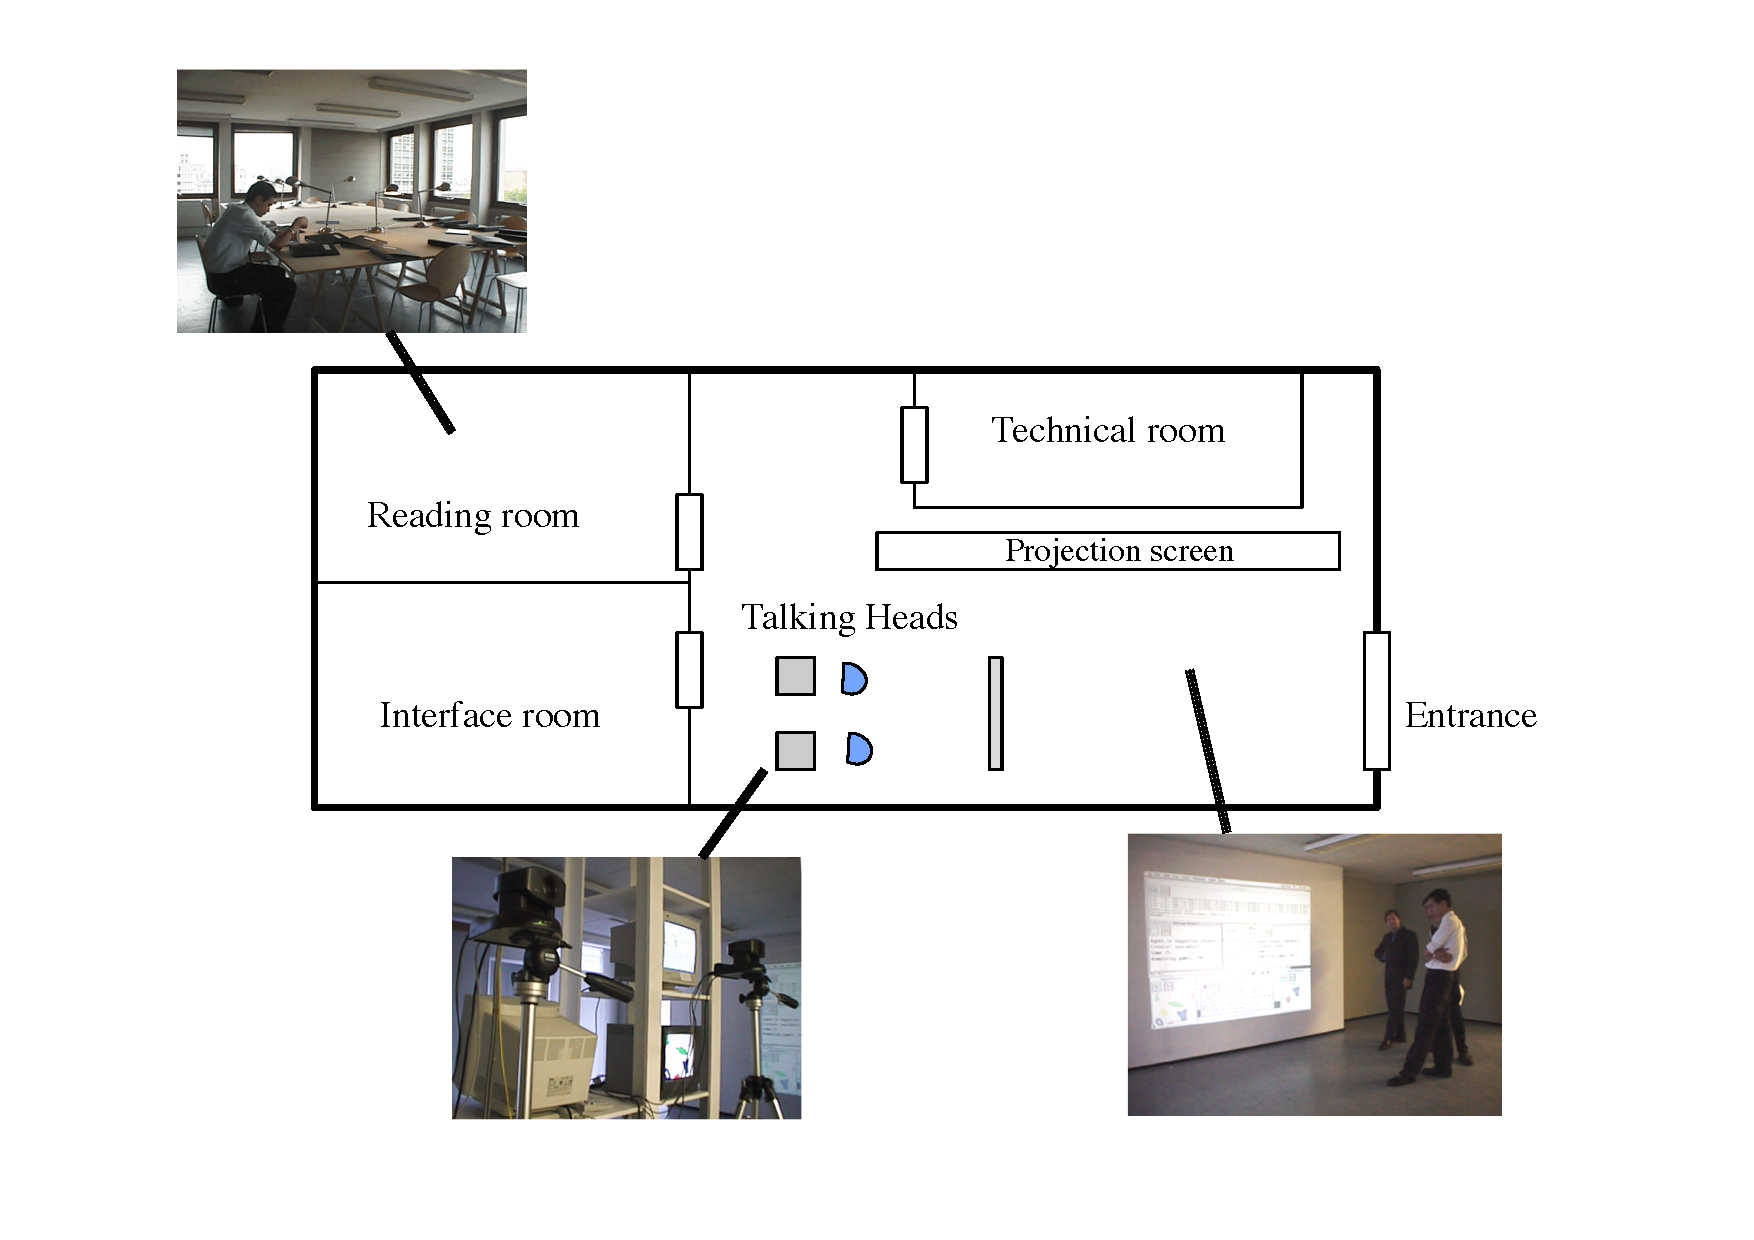
\includegraphics[width=0.9\textwidth]{chap8/figures/layout}}
\caption{\label{fig:layout} 
Layout of the 'Laboratory for Cognitive Robotics and Teleporation" at the Laboratorium exhibition in Antwerp.}
\end{figure}


\begin{figure}[htbp]
 \centerline{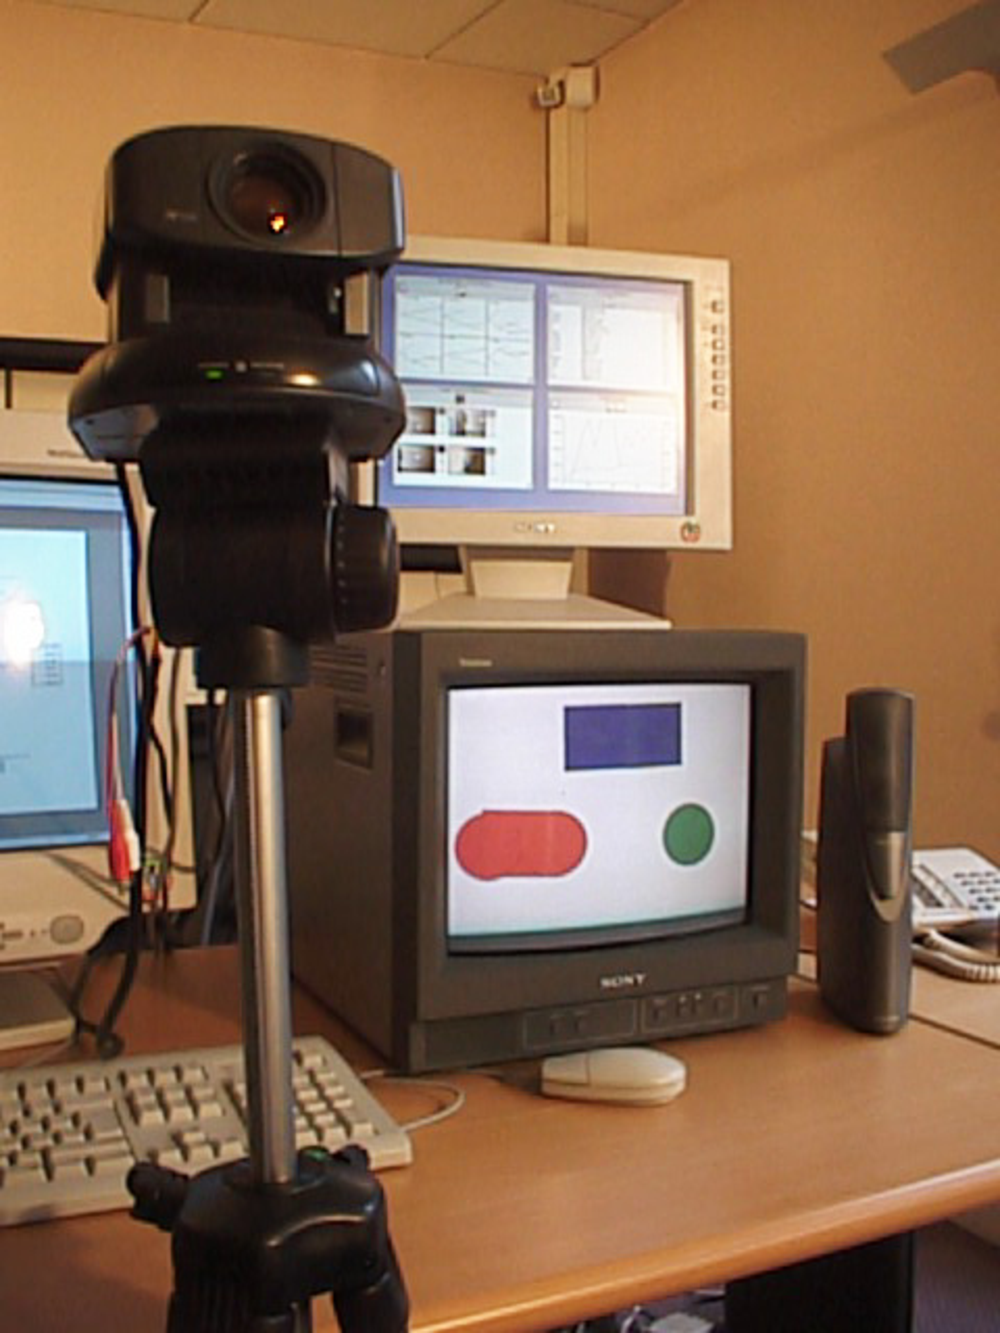
\includegraphics[width=.35\textwidth]{chap8/figures/zoom-in-head}}
\caption{ \label{fig:laboratorium} 
A single Talking Head at the Paris site. In the background we see (bottom) the display with an
image that the agent picked up, (on top of that) a screen displaying the processed image and the discrimination trees, 
and to the right the loudspeaker broadcasting the speech output of the agent.}
\end{figure}

A typical example of the kind of images that the camera's picked up are shown in \figref{fig:images}. 
To play a game, the agent had to find a sufficiently delineated group of objects and each object had 
to exceed a minimal size. Initially quite complex configurations were put on the white board but this made it very difficult for agents to find a coherent group and to develop good concepts for referring to the topic. The right 
image in \figref{fig:images} provides clear examples of up, down, left and right, different colors, and 
also opportunities to use multiple words (such as ``red bottom"). 

\begin{figure}[htbp]
 \centerline{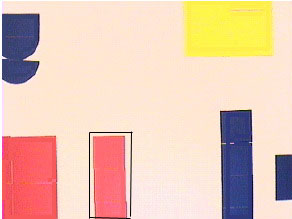
\includegraphics[width=.40\textwidth]{chap8/figures/image-1}
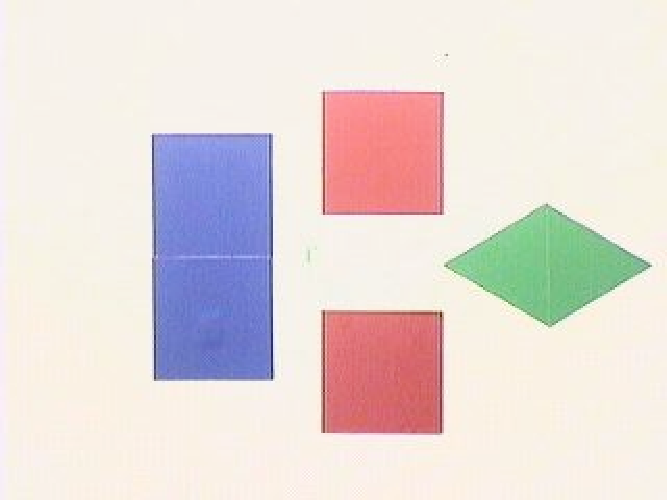
\includegraphics[width=.40\textwidth]{chap8/figures/image-2}}
\caption{\label{fig:images} 
Examples of images picked up by the camera's. The chosen topic was signalled by drawing a bounding box around it. 
During experimentation, it was found that configurations such as in the right image lead to more stable performance.} 
\end{figure}

A typical example of an interaction is shown in \figref{fig:interaction}. 
The speaker (called "rubber", an agent created and named by a user) has selected the blue object at the bottom left 
of the screen. We see the discrimination trees of the agent at that point and the data for each of the objects 
recognised. The coordinates of the respective objects (scaled within the coordinate system of 
the captured image) are (0.0,1.0) for the blue object, (1.0, 0.96) for the red one, and (0.42, 0.0) for the green one. 
The values are displayed as HP (horizontal position), VP (vertical position), H (height), W (width), A (area), 
R (red), G (green), Y (yellow), B (blue), L (lightness). 
The blue object is chosen as the topic and the value on the blue channel has the most discriminative power, although 
there are other possibilities. There are three competing words for naming blue: Xagadude, Nibidesu, and Tetipi. 
None of them have a score higher than 0 and so a random choice of Xagadude is made. 

The hearer (called "me") perceives an image which is slightly different from 
the one seen by the speaker. Also the discrimination trees built up so far by this agent are different from the ones used
by the speaker. The hearer does not know the word, so the game fails. After the speaker has then pointed to the 
topic, the hearer conceptualises and guesses that the meaning of this word is 'blue' because that is also for him the most 
discriminating feature of the topic (which has coordinates 0.0, 1.0) compared to the other objects in the context. 


\begin{figure}[htbp]
 \centerline{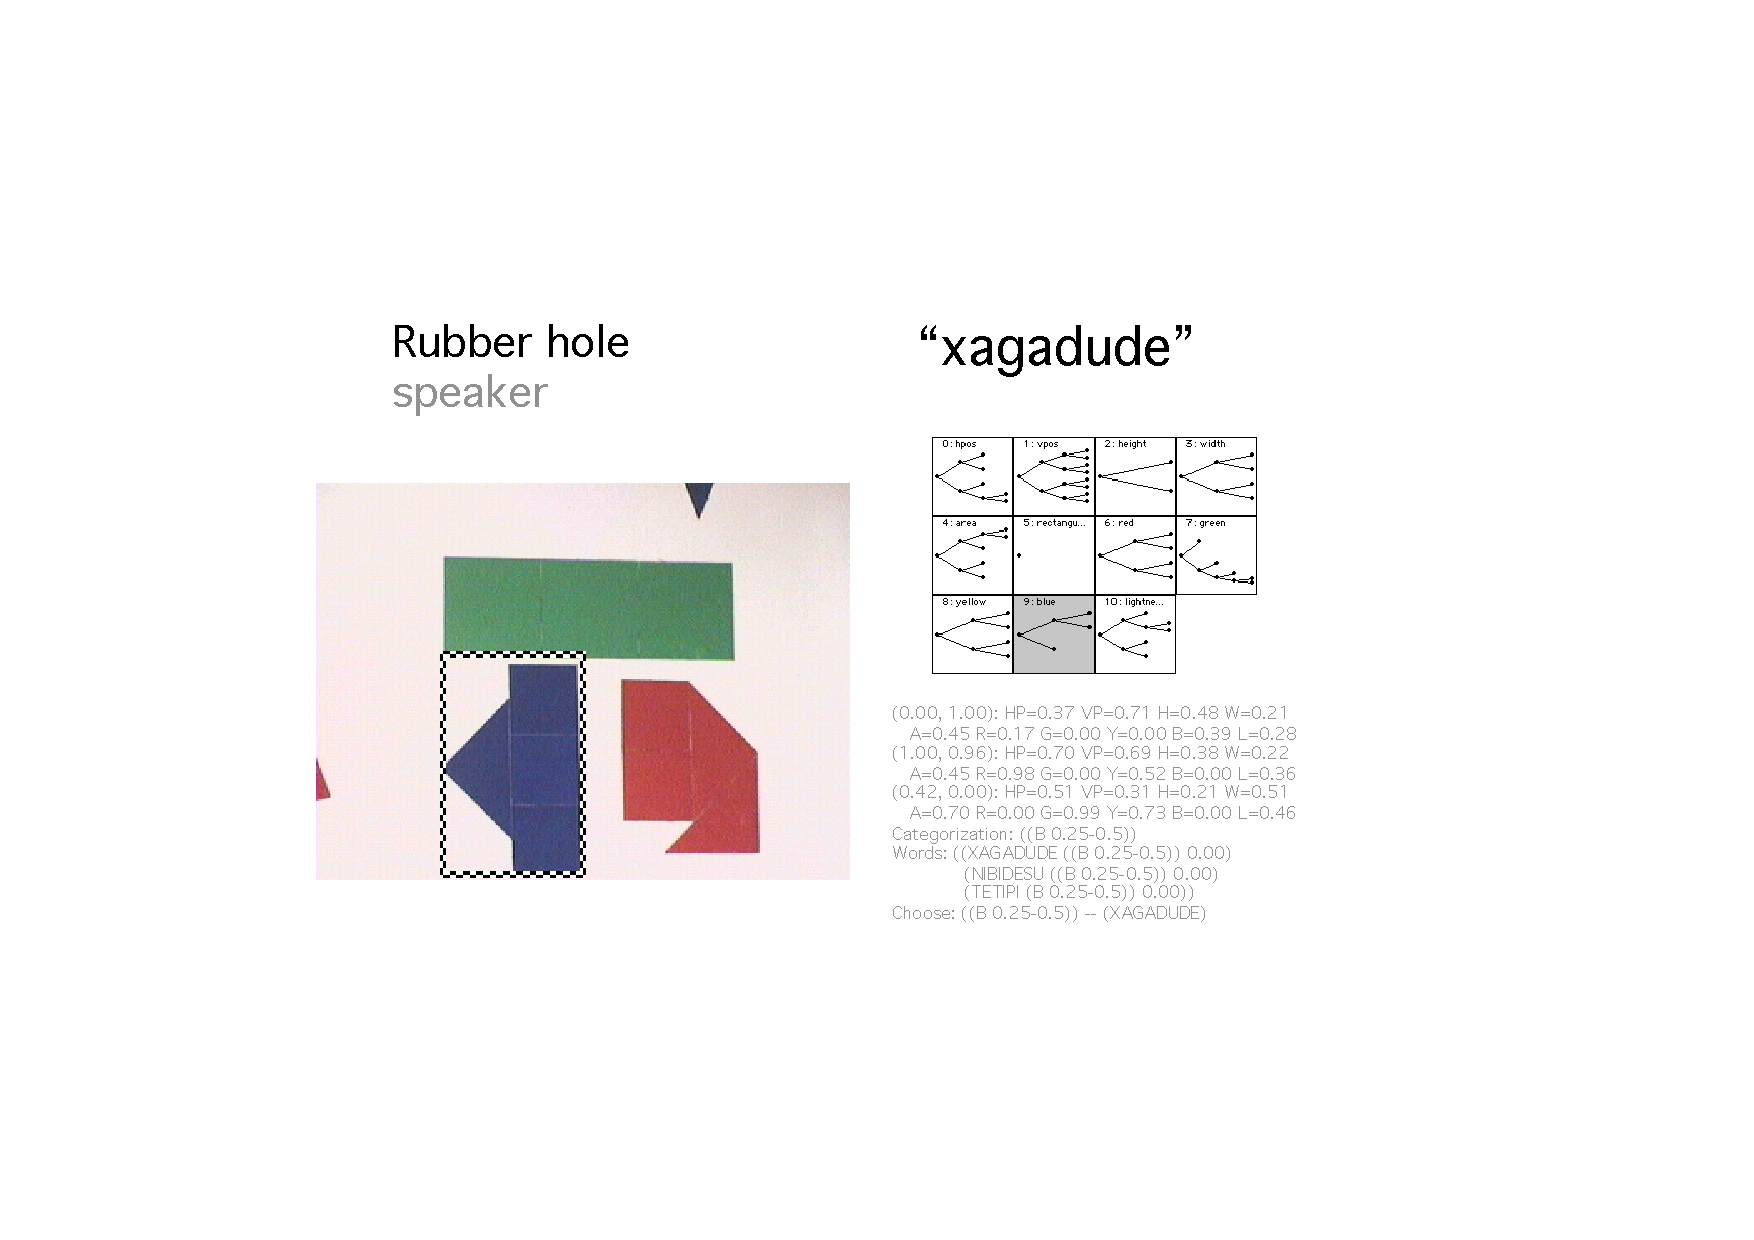
\includegraphics[width=.80\textwidth]{chap8/figures/xagadu-speaker}}
\centerline{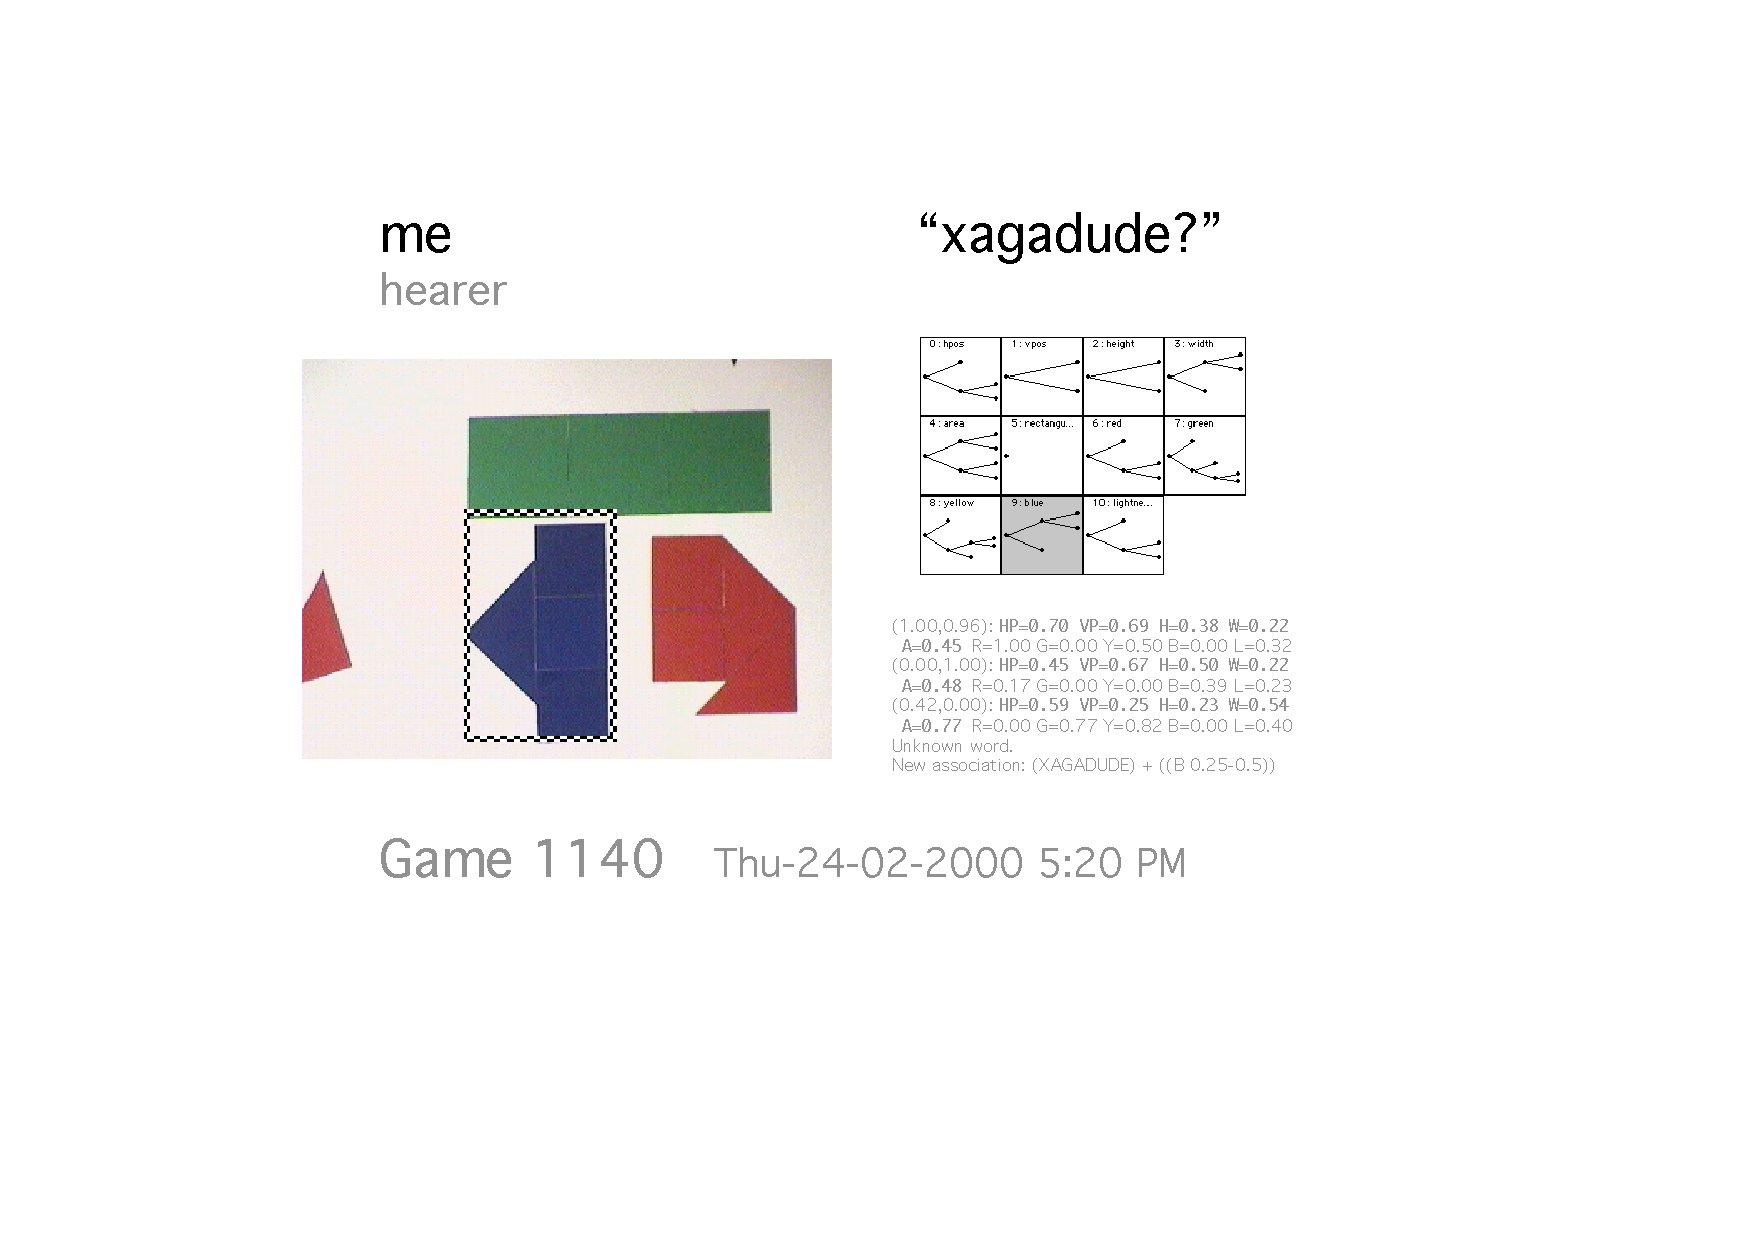
\includegraphics[width=.80\textwidth]{chap8/figures/xagadu-hearer}}
\caption{\label{fig:interaction} 
Top: Source image, conceptualisation, and word choice of the speaker. Bottom: Source image, parsing and interpretation 
of the hearer.}
\end{figure}

The experiment had also a presence on the web, designed by Angus McIntyre. Anyone could log in on the 
Talking Heads website\is{Talking Heads website}, create an agent with 
a given name, and launch it on a tour of the various physical sites. There was also a forum on which users could discuss
the experiment as it was progressing, a hall of fame for the agents that were the best communicators, and 
an overview of the lexicon 
that had formed so far. The website allowed inspection of what was happening at each site (\figref{fig:thwebsite}): 
Users could check which agents were waiting there to play a game, and what the current 
game was about. It displayed also statistics about the 
communicative success and agent activity at each site. The site is no longer operational due to 
changes to the underlying software but some remnants can be visited here: https://ai.vub.ac.be/talking-heads/

\begin{figure}[htbp]
  \centerline{
\includegraphics[width=.85\textwidth]{chap8/figures/th-website}}
\caption{\label{fig:thwebsite} 
The Talking Heads website main interface. Users could create and manage their own agents and inspect what was happening 
at each site. Here 12 agents located at the Brussels site are listed.}
\end{figure}

An example of how the web interface displayed a single game is shown in \figref{fig:thwebsite-agent}. 
There are two agents: Antonusius is the speaker and Zelebot is the hearer. 
The green object has been chosen as topic and correctly 
recognised by the hearer using the word ``kazozo". The meaning of the word was not visible through the interface because we 
wanted users to learn themselves the language of the agents. 


\begin{figure}[htbp]
  \centerline{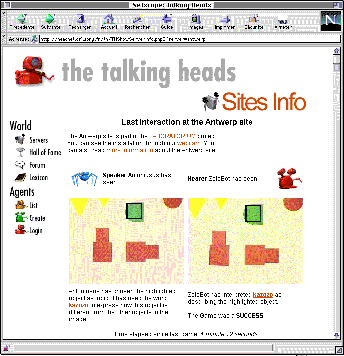
\includegraphics[width=.85\textwidth]{chap8/figures/zelebot}}
\caption{\label{fig:thwebsite-agent} 
Example of an interaction that took part in Antwerp. This game was a success. The agents recognised the same
set of objects and the meaning of ``kazozo" was effective in finding the same topic. 
}
\end{figure}

\section{Start up of the experiment} 

Once the physical installation at the Antwerp site was completed, work focused on getting the experiment itself 
up and running. It is interesting and instructive to look at some snippets of the email correspondence during the 
first weeks. The despair when trying to cope with the unavoidable problems but also the excitement 
as a language began to emerge shines through. The English humor of Angus McIntyre was a welcome antidote to 
all the stress. The correspondence reprinted here is a small selection but also necessary fragmentary because a 
lot of communication took place face-to-face or through the telephone, as email was not always possible. 

We pick up the email correspondence on
June 23, 1999 when the first experiments are taking place to try and make language games at the three sites possible 
and allow the scheduling and activation of agents. 

\subsection*{23 June 1999}

\begin{mail}
--============\_-1278188520==\_d============\\
From: Angus McIntyre <angus@csl.sony.fr>\\
Subject: Re: Brussels is back\\

At 9:04 pm +0200 23.06.99, Joris Van Looveren wrote:
>Brussels is officially back on line. I forgot to make sure that there
\\>were no agents here before I launched it, so don't be surprised if it
\\>turns out that some agents have suddenly been cloned :)

I don't think agents can be cloned; 'headnet' will probably just 
say "Oh, back so soon?" and overwrite existing definitions. This 
may lead to inconsistencies if two copies of an agent are out 
and about at the same time ...

Brussels is active, which is good. Paris appears to have gone 
to sleep, either because the lights are out, or because it's 
past its pre-defined bedtime. Still, the Babel software still 
seems to be running with nothing more than the usual email process errors.

>- The machine is still fast enough to do other work. The only
\\>  thing that is a bit annoying is that it stalls when images
\\>  are being grabbed (read: sent over the bus).

There's a lot of data moving over a slow line, and evidently 
the MacOS is giving it priority to prevent dropped frames 
when doing video capture.

>- Since there is no sound, it is blazingly fast compared to
\\>  the Antwerp installation (2-3 games per minute or so)

Speech and camera motion are the big slow downs. This means that 
we're not under a lot of pressure to optimize the agent code, as 
the agents can do all their discriminations faster than we'll 
ever be able to drive the cameras (until we try using the little 
EVI-G21's, which only have to move a little CCD unit rather than 
a whole camera assembly, and apparently track very quickly indeed).

I've announced the site to a handful of links pages (Peter Norvig's 
AI links collection, Chris Bogart's Constructed Languages page, the 
NASA real robots page - links to all these sites are under 
'background' on our site). I haven't yet done a massive submit of 
the site to the big search engines or announcement sites; I suggest 
that we let traffic build slowly so we can find out what we can handle.
	A
\end{mail}


\subsection*{24 June 1999}

The (faster) machines that were planned are now available, so that a switch has to be made while the 
experiment is already running. 
\newline
{
\begin{mail}
--============\_-1278188520==\_d============\\
From: Angus McIntyre <angus@csl.sony.fr>\\
Subject: 'headnet' now running on new PII 400 server.\\

Silvere and Alexis have installed Linux and the headnet software on the 
new 400Mhz Pentium II server, and I've done the DNS switch (and updated
/etc/hosts, and csl.zone, and sony.rev, and sony.zone, and killed half 
a dozen in.named processes, and killed squid, and restarted 
squid, and killed squid, and restarted squid, and killed squid, 
and deleted squid's cache, and restarted squid, and flushed my Netscape
cache, and flushed everyone else's Netscape cache, and flushed the 
Netscape cache of eight dozen people in Australia who I've never 
met, and individually inspected and edited every packet on the 
Internet to make sure that 'headnet.csl.sony.fr' now points to the new box).

The result of this is that 'headnet.csl.sony.fr' should now get 
you the P400 server, and 'headnet-dev.csl.sony.fr' should get you the 
old 200Mhz Vectra, which can be recognised because it has the words 'test 
site' in the banner that appears at the top of the page.

With luck, the change should be transparent and you shouldn't need 
to do anything. You should however check to make sure that your agents 
are going to the right server, however, and that when your browser looks 
for 'headnet', that it gets the correct machine. If your Babel server 
accesses 'headnet' via a cacheing proxy server, you may also need to 
ask your sysop to clear the server's cache and restart it.

Enjoy 
A
\end{mail}
\begin{mail} 
--============\_-1278188520==\_d============\\
To: Joris Van Looveren <joris@arti.vub.ac.be>\\
From: Angus McIntyre <angus@csl.sony.fr>\\
Subject: Re: Brussels 2pm\\

At 2:00 pm +0200 24.06.99, Joris Van Looveren wrote:
>We're planing to go to Antwerp in 1 hour. There is no telephone there,
\\>so we will communicate by email ... We're thinking of clearing the 
\\>database around 4 pm. ... do you want to do it from Paris ?

You do it. At 3:55pm, I'll kick all the agents off 'paris' and pause it. 
When I see headnet has been cleared, I'll restart 'paris' and make 
some new agents.

I'll upload the changed TH website with the direct links to 'headnet' 
at the same time.

		A
\end{mail}
\begin{mail}
--============\_-1278188520==\_d============\\
From: Angus McIntyre <angus@csl.sony.fr>\\
Subject: Things to do in Antwerp when you're head(net) ...\\

There seems to be some problem with the changeover of the machines. 
What's happened is that the new address for 'headnet' (193.105.194.10, 
which is to say the PII 400, rather than 193.105.194.8, which is 
the Vectra formerly known as 'headnet' but now 
represented by an unpronounceable symbol that means 'headnet-dev') has not 
yet propagated through the DNS as far as Belgium.

So Antwerp (yeah! welcome to the net!) is sending its agents to 'headnet-dev', 
rather than 'headnet'. There's no great problem here as far as testing your 
installation goes, except that 'paris' is pointing at the new 'headnet' and 
'brussels' is apparently dead, so you won't be seeing any foreign agents.

In theory, if you reboot, the DNS results cached on the Macintosh should go 
away, forcing a re-lookup which ought to get the correct values. If that 
doesn't work, you could try taking the MacTCP DNR file which lives in the 
System Folder *out* of the System Folder and then rebooting. And if that 
doesn't work, we just have to be patient and wait for the changes to propagate. 
You could also consider entering the address of 'headnet' as dotted IP 
(193.105.194.10) in the network configuration dialog.

	A
\end{mail}
\begin{mail}
From: Angus McIntyre <angus@csl.sony.fr>\\
Subject: Re: Database cleared\\

At 5:47 pm +0200 24.06.99, Joris Van Looveren wrote:
>The databases have just been cleared. You can create new agents now.
\\>Brussels might be down for some more time, so check if it's up before you
\\>send any agents there.

OK. I notice there are bugs in the server code which cause it to 
generate scads of errors when the database is empty, but those should clear.

I've restarted 'paris', and I'm now going to make some agents to 
send there. Antwerp is showing up on 'headnet', and the error 
messages strewn all over the site should go away when we get 
some data into the database.

When it begins to look a little more solid, I'll upload the 
changed pages on 'talking-heads', and then we'll really be live.

	A
\end{mail}
\begin{mail}
From: Angus McIntyre <angus@csl.sony.fr>\\
Subject: Re: Webcam\\

At 6:28 pm +0200 24.06.99, Joris Van Looveren wrote:
>The Antwerp webcam is on-line:

I've added a link from the Antwerp page on the main site, 
and I've also added a link in the descriptive text about 
the Antwerp server which appears on the 'server overview' page. 

I actually saw one of you - Fred? - through the Antwerp 
webcam a moment ago.

> Also, the Antwerp and Brussels site are up 'permanently', 
\\> so can send agents to them.

I've created a bunch of agents and sent them round the sites. 
The server seems to be acquiring consistency.

I'm off home now. If you need me to come back and kick 
the server, call me on:
	+33-1-42-78-73-88
Bye,
	A
\end{mail}
}

\subsection*{25 June 1999} 

The different sites and the teleportation infrastructure are now running but there are still basic problems 
stemming from hardware and software glitches. 


\begin{mail}
--============\_-1278188520==\_d============\\
Date: Fri, 25 Jun 1999 05:13:55 EST\\
From: "frederic kaplan" <fred@captage.com>\\
Subject: First night\\

The talking-heads in Antwerp have passed the night OK... 
34 agents
18 users... It goes fast

It seems that Paris and Brussels are not playing anymore ?

Fred.
\end{mail}

\begin{mail}
From: Angus McIntyre <angus@csl.sony.fr>\\
Subject: Re: Antwerp \& Brussels live!\\

At 10:52 am +0200 25.06.99, Joris Van Looveren wrote:
>I got e-mails from Antwerp and Brussels that they resumed normally this
\\>morning. So they both survived their first night on the job!

Paris seems to be still ticking along. One thing I notice is that it's 
quite easy for agents to 'pool' on one particular server at the expense 
of others. The more agents you have on any one server, the longer it 
takes for each agent to get through its assigned 50 games or whatever. 
So servers with many agents tend to stay occupied, and others which are 
waiting to receive agents can often stand empty waiting for the agents 
to play out their games on the crowded servers.

It's probably a good idea to have a few agents (either the ones owned 
by 'adm' or your own agents) set up to make round trips, playing five 
games here, five games there, and so on. Long routes of small numbers 
of games rather than short routes involving many games is probably 
the way to load balance and prevent servers drying up.

> ... the database is still accessible through a simple URL,
\\>without any protection (password). I think since headnet has gone
\\>public, it would be a good idea to change this ...

The same idea had occurred to me. I'll look into that (trans: I'll 
try to find the piece of paper on which I wrote down the root password 
to 'headnet' and, if I find it, I'll set up an .htaccess 
file to keep strangers out).

I've told a few friends of mine about it, and the response 
so far has been generally positive, although Sylvia - Luc's 
proofreader - apparently has some reservations about the 
usability of the site.

Hmm. News update.

A friend of mine, who shall be nameless, sent down an agent with route:
	'brussels paris antwerp'
As I predicted a few days ago, this will (and did) cause a 
LISP-level error.

I patched the route by hand and then made the mistake of trying to use 
MCL's rather flaky 'Restart frame' option to go on. At first this seemed 
to have worked, but about one game later things went bad and the whole 
machine locked. One of the three agents then on the server managed to 
get out just seconds ahead of the meltdown, but two more were caught 
on the server and are now in limbo. I've edited the database for one 
of them to try to resurrect it, and if that works, I'll try to 
revive the other as well.

I'll also write a quick bit of code to do route-checking to try 
to make sure that this doesn't happen again.

	A
\end{mail}

\begin{mail}
--============\_-1278188520==\_d============\\
From: Angus McIntyre <angus@raingod.com>\\
Subject: The Lazarus Syndrome\\

When a Babel server falls over and agents get lost, it's possible to 
restore them to life by going onto Headnet's 'admin' page and editing 
the agent's entry in the 'THAgent' table. Basically, if you reset 
the 'isonserver' field to 1 (it will be 0 when the agent's away), 
the agent should spontaneously reappear on headnet and then move 
off to wherever it was meant to go.

There will be inconsistencies in the database - 'headnet' will 
remember all the words that the agent used before the crash, but 
the agent's own memory is reset to what it was when it left 'headnet' - 
but with luck they shouldn't be too serious.

By the way, there's a bug in the 'headnet' software with respect to 
routes; there's a finite limit on the field length for the 'route' 
field. If you make a route that's too long, it gets truncated, so 
you can have an agent whose route goes:
	... paris 10 bruss
The agent will complete its games on 'paris' and then go into 
stasis waiting for a server called 'bruss' to pick it up. A patch 
for this would probably be nice to have at some point.

	A
\end{mail}

\begin{mail}
--============\_-1278188520==\_d============\\
From: Holger Kenn <kenn@arti9.vub.ac.be>\\
Subject: Alpha box in Antwerpen gone...\\

Hi !

The alpha box in Antwerpen is gone.

Please somebody reboot it ASAP, or we won't have a connection to
Antwerpen anymore...

Holger
p.s.: 
To reboot: 
	Disconnect Printer.
	Switch alpha box off.
	Switch on again.
	Wait about 5 Minutes.
	Reconnect printer.

Holger
\end{mail}

\subsection*{28 June 1999} 

After the basic hardware appeared to be operational, attention turned to the actual behavior of the 
emergent language system. Initial results are not very encouraging. 

\begin{mail}
--============\_-1278188520==\_d============\\
From: Luc Steels <steels@arti.vub.ac.be>\\
Subject: paris site \\

I just examined the Paris site a bit. The error rate is
distressing. This is due to many things.

1. The calibration is way off. Even if they get it
right, calibration mixes up completely the game.
It is obligatory to calibrate much better tomorrow
morning (can you do this frederic?)

2. The light conditions were very bad and have been improved a bit so that 
patches of white light are no longer seen as objects.

3. The visual situations about which the agents are playing games
are way too complex. Even humans would not be able to play the game. I simplified
enormously. We need to make similar clear situations AT ALL sites so that the 
agents can really learn the very basic concepts first. Also salience
might have to be set lower to have multi-categories and consequently multi-words
(although there is a fundamental bug in the multi-word thing it seems). Now the
agents are making much too deep discrimination trees because of the confusing 
nature of the situation and the errors in pointing. If the top agent 
only has 20 % right after a few days there is something fundamentally wrong 
in the setup because it is pure chance. The fact that success drops means 
that self-organisation is NOT taking place.

4. We might have to change the word creation rate to be less than 1.0. 
In the present circumstances I believe that every agent will make for every node
in the tree at very great depth his own word.

I suggest that tomorrow we go through games with the agents step by step and fix 
the environment and the lights, etc. so that the game is at least feasible; at the 
moment it is not. The same exercise will have to be done in Brussels and Antwerp. 
There is a question how we can get rid of all the garbage that is being created right now.

luc
\end{mail}

\begin{mail}
Date: Tue, 29 Jun 1999 13:07:48 +0200\\
From: Joris Van Looveren <joris@arti.vub.ac.be>\\
Subject: Re: paris site\\

Luc Steels wrote:
> 2. The light conditions were very bad and have been
\\> improved a bit so that patches of white light are
\\> no longer seen as objects.
The problem is reflections on the whiteboard. In brussels the lights are
covered so that there is no direct light falling onto the whiteboard.
Consequently, it happens rarely if ever that parts of the background are
seen as objects.

Also, turn on the 'back light' option of the cameras. This improves the
image quite a bit, especially at lower light intensities. I'll try to
find out if it can be turned on and off from software, so that the
setting can be saved along with the other configuration data.

Joris.
\end{mail}

\begin{mail}
--============\_-1278188520==\_d============\\
From: Luc Steels <steels@arti.vub.ac.be>\\
Subject: Major error in feedback \\

Based on the dismissal performance in Paris, we
discovered a major error in the feedback. I
suggest that all sites at this point PAUSE until
we fix this and then we update versions on
different sites. This bug may explain why
the lexicon has disintegrated.

more news soon.

luc
\end{mail}

\subsection*{29 June 1999} 


\begin{mail}
--============\_-1278188520==\_d============\\
Date: Tue, 29 Jun 1999 11:38:23 +0200\\
From: Joris Van Looveren <joris@arti.vub.ac.be>\\
Subject: Antwerp OK\\

Antwerp has not been down, contrary to what the server page showed. The
problem whas that the network was not accessible any more because the
network interface of the alpha machine was down. This meant that the
proxy was not available. According to Mario, the games have continued,
so probably in a couple of hours when all interactions and agents have
been uploaded, the database will be up to date again. 

At this moment, Brussels and Paris have been paused until further
notice. Interactions continue to be uploaded until the network interface
has caught up.

Joris (in Brussels) \& Mario (in Antwerp).
\end{mail}

\begin{mail}
--============\_-1278188520==\_d============\\
Date: Tue, 29 Jun 1999 16:35:46 +0100\\
From: Frederic Kaplan <kaplan@csl.sony.fr>\\
Subject: Patches\\

Bugs fixed

1. Feedback mechanisms and find-segmented-pointed by the hearer (this
was not working at all...) corrected in: segment-tools.lsp and th-world.lsp

2. scaling. If a value is higher than the maximum, it gives max as opposed to
1.0!!! corrected in: geom.lsp

3. Masking. Eliminating zero channels should be done on the source not on
value (= value after scaling, so it is often zero). corrected in: 
prototype.lsp (in the functions folder)

After theses patches, sites can be running again.

Fred and Luc.
\end{mail}

\begin{mail}
--============\_-1278188520==\_d============\\
Date: Tue, 29 Jun 1999 23:25:45 +0200 (MET DST)\\
Subject: There is hope for robokind \\

After fixes to the Paris site by Frederic and me, I relaunched some agents. 
Things are now beginning to work as they should. We can see the
agents quickly build up a successful lexicon.

It is a pity that at the moment one can no longer give more 
than 20 games (although I can see the goal of getting to a global 
coherent lexicon that way). I try to circumvent by immediately
sending them 3 times to Paris but I am not sure this works.

Brussels and Antwerp should wait until all the fixes have been made 
before re-entering the network. Frederic and I will send a mail tomorrow
morning. Once the system works, it is quite exciting to see your agents move 
forward quickly!

Luc
\end{mail}

\subsection*{30 June 1999} 


\begin{mail}
============\_-1278188520==\_d============\\
Date: Wed, 30 Jun 1999 11:16:41 +0200 (MET DST)\\
From: Luc Steels <steels@arti.vub.ac.be>\\
Subject: progress \\

The mails to talking-heads go in a log file and I suggest that everybody not 
only sends technical issues but remarks.

The Paris site is really taking off now. A lexicon is beginning to 
be in place, mostly focusing on positional information (left, right, up, 
down). Because the lexicon is getting established, it is now easier for
new agents to acquire the existing lexicon and be successful. The agents have less
bushy discrimination trees and fewer but effective words. This was demosntrated
by frederic's agent (Kant) which quickly came to the top as speaker after only a
few games!

The word "green" apparently means red. So I am teaching my agents the word
rouge instead of green. It is not yet clear to me whether you can influence 
the lexicon once it is already firmly established.

Later this afternoon we might enrich the agents' experiences by changing the
environment a bit.

Luc
\end{mail}

\begin{mail}
--============\_-1278188520==\_d============\\
Date: Wed, 30 Jun 1999 17:16:19 +0200\\
From: Joris Van Looveren <joris@arti.vub.ac.be>\\
Subject: Re: paris site\\

Luc Steels wrote:
> 4. We might have to change the word creation rate to be less than 
\\> 1.0. In the present circumstances I believe that every agent will 
\\> make for every node in the tree at very great depth his own word.

Don't do this yet. It will cause the system to crash sooner or later, as
I experienced in Antwerp and Brussels today. The reason is the method
utterance-word-string is not defined on null-utterances. I'm trying to
find out what result this method should return.

I've been in Antwerp today to get it running again and to apply the
patches. It had run well for quite some time when I left, but something
caused it to crash again half an hour later. I'll try to fix it tomorrow
with Mario, if he has the time to go there.

Joris.
\end{mail}


By mid July, both the basic infrastructure, the teleportation mechanisms and the semiotic dynamics were running 
smoothly and so the experiment could operate without constant care. 

\section{Results of the experiment}

The first `Talking Heads' experiment ran for 4 months during the summer of 1999 and showed the validity of the mechanisms that were used for the agent architecture and of the interaction patterns and group dynamics of the agents. A shared lexicon and an underlying conceptual repertoire emerged, enabling successful communication by the agents about the scenes before them. In total, 400,000 grounded games were played. The population of agents rose to just under 2000, increasing steadily over the period of the experiment. Despite the many perturbations due to grounding, intermittent technical failures, a continuous influx of new agents entering the population, and unpredictable human interaction, the lexicon was maintained throughout this period.

The rate of communicative success for the first 200,000 games is shown in \figref{fig:allsites}. We see that the successrate is generally between 70 and 80 \%. There are occasionally crashes (e.g. around 90,000) caused by problems at a particular site (such as bad light conditions). 


\begin{figure}[htbp]
  \centerline{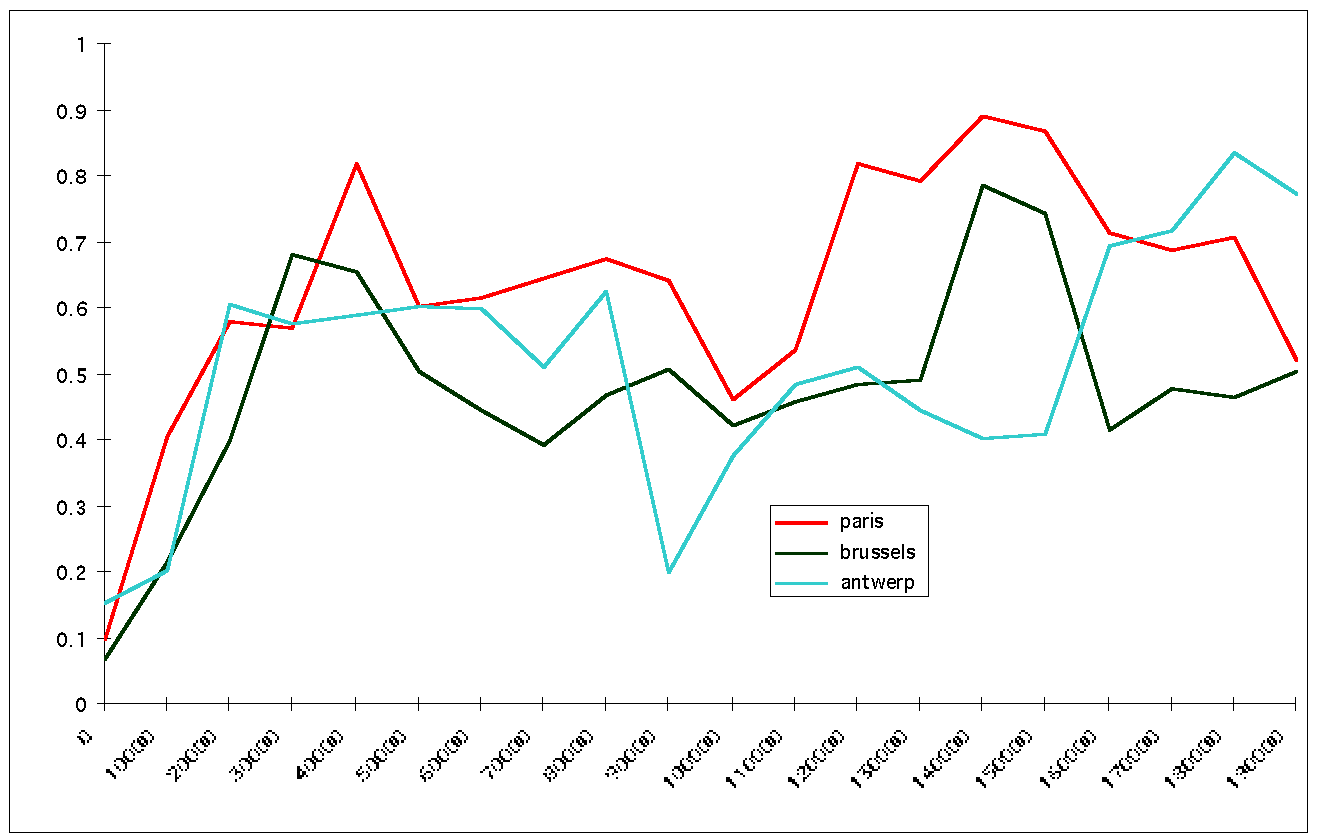
\includegraphics[width=.80\textwidth]{chap8/figures/allsites}}
\caption{\label{fig:allsites} 
The y-axis shows the average communicative success of agents at each of the three different sites for a total 
of 190.000 games shown on the y-axis. 
}
\end{figure}

A total of 8000 words and 500 concepts were created by the agents, with a core vocabulary consisting of 100 basic words expressing concepts like up, down, left, right, green, red, large, small, etc. Of these, 8 words represent a large majority of words used (about 80 \%). 4 of these words refer to the position of objects: GOREWA (top), DOWN (bottom), WOGGLESPLAT (left), and SESUBIPU (right). 4 other words refer to colors: ROUGE (red), KAZOZO (green), WEGIRIRA (blue), and EMPTY (light). The distribution of these words after 130,000 games is shown in \figref{fig:words-used}. 


\begin{figure}[htbp]
 \centerline{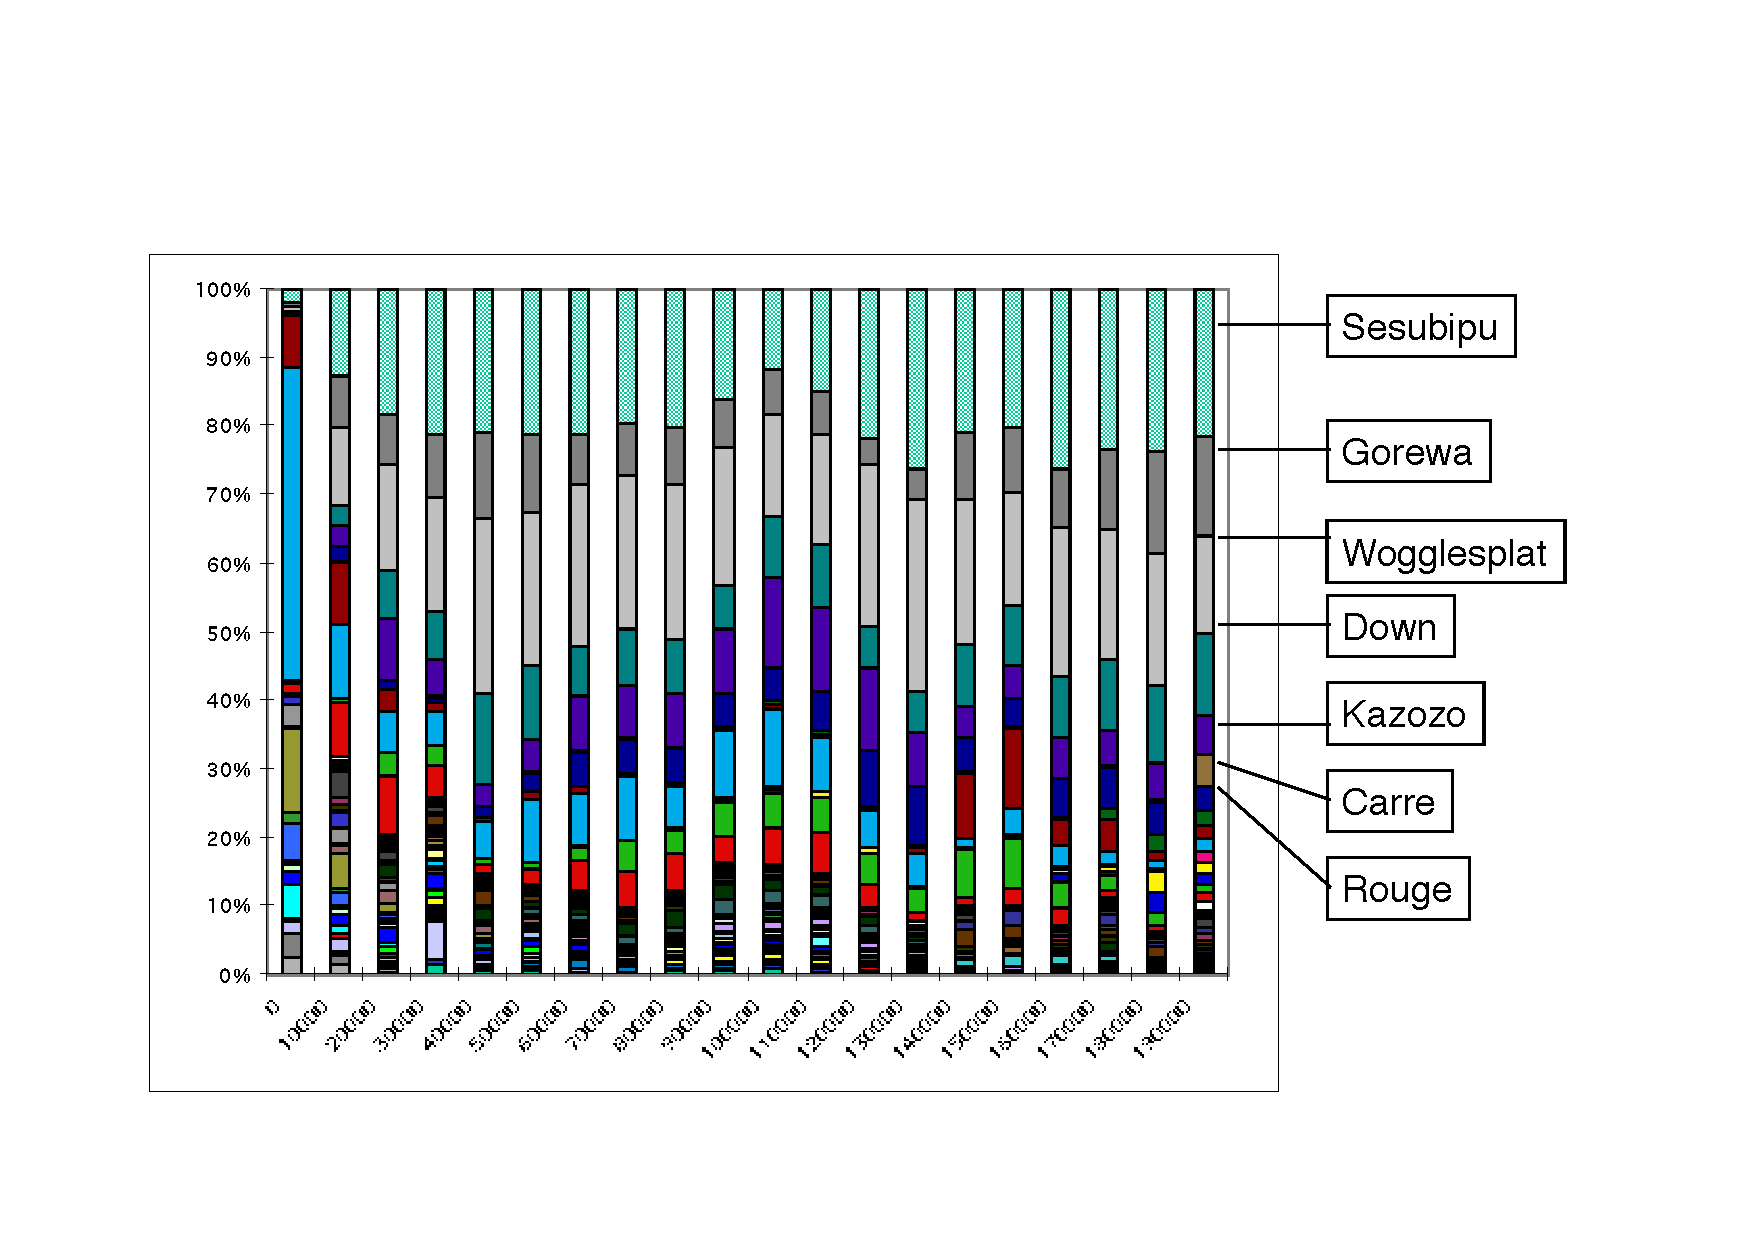
\includegraphics[width=.80\textwidth]{chap8/figures/words-used}}
\caption{\label{fig:words-used} 
Distribution of word use. There are only a few words that are dominant. Many words are 
short-lived, either because the circumstances 
in which they fit are rare or because they do not get settled in the population. Moreover sometimes users create agents 
which they do not keep rescheduling for new games. 
}
\end{figure}

\figref{fig:woggle} shows the semiotic dynamics related to an expression of the meaning for the 
concept `left', i.e. a horizontal position 
between 0.0 and 0.25 (after scaling). The word "wogglesplat" becomes dominant
although there is a very strong competition in the beginning. 
We see that users try to give other words to the same meaning, such as "gauche" or "links" (both words expressing left 
in French and German or Dutch respectively). We also see that other words such as "red" or "yellow" get associated with this 
meaning, because the hearer may guess the wrong meaning in learning the word for left. 

\begin{figure}[htbp]
  \centerline{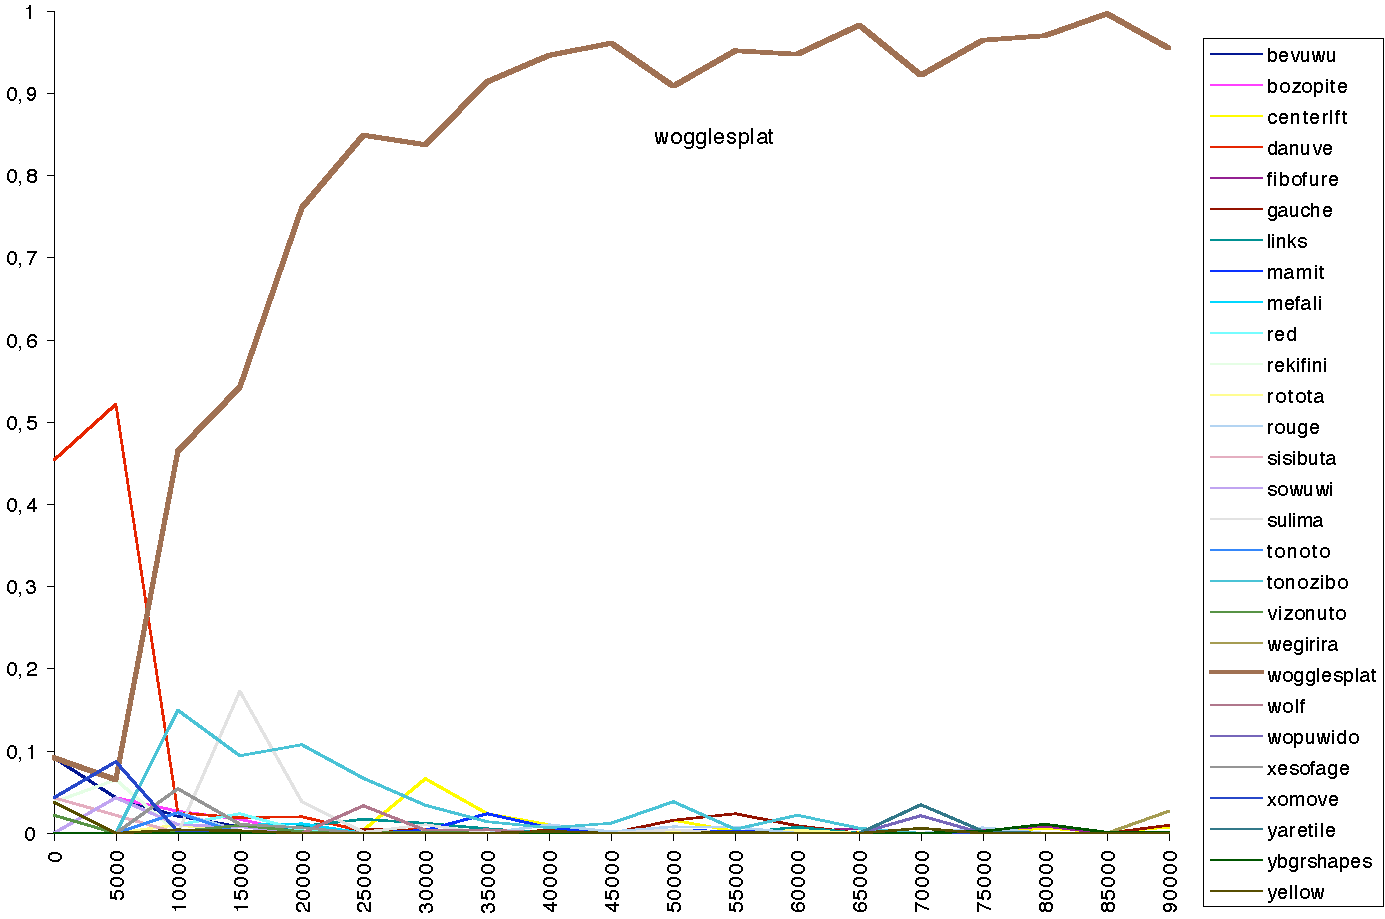
\includegraphics[width=.80\textwidth,height= 6cm]{chap8/figures/wogglesplat}}
\caption{\label{fig:woggle} 
Meaning-Form diagram: Different words for expressing the meaning 'left', i.e. 
horizontal position is less than 0.25 (scaled). 
New words come up all the time but there is a clear winner-take-all effect with "wogglesplat" winning. 
}
\end{figure}

\figref{fig:droite} shows another example of the semiotic dynamics in the experiment, this time looking at all the 
meanings for a particular word, namely ``droite" (meaning `to the right' in French). This word clearly has been introduced
by a human user and the dominating meaning progressively becomes a region (between 0.75 and 1.0) on the horizontal position, 
as could be expected. On the way we see some confusion, Specifically there must be objects that appear both on the right 
and up (vertical position between 0.5 and 1.0). 

\begin{figure}[htbp]
  \centerline{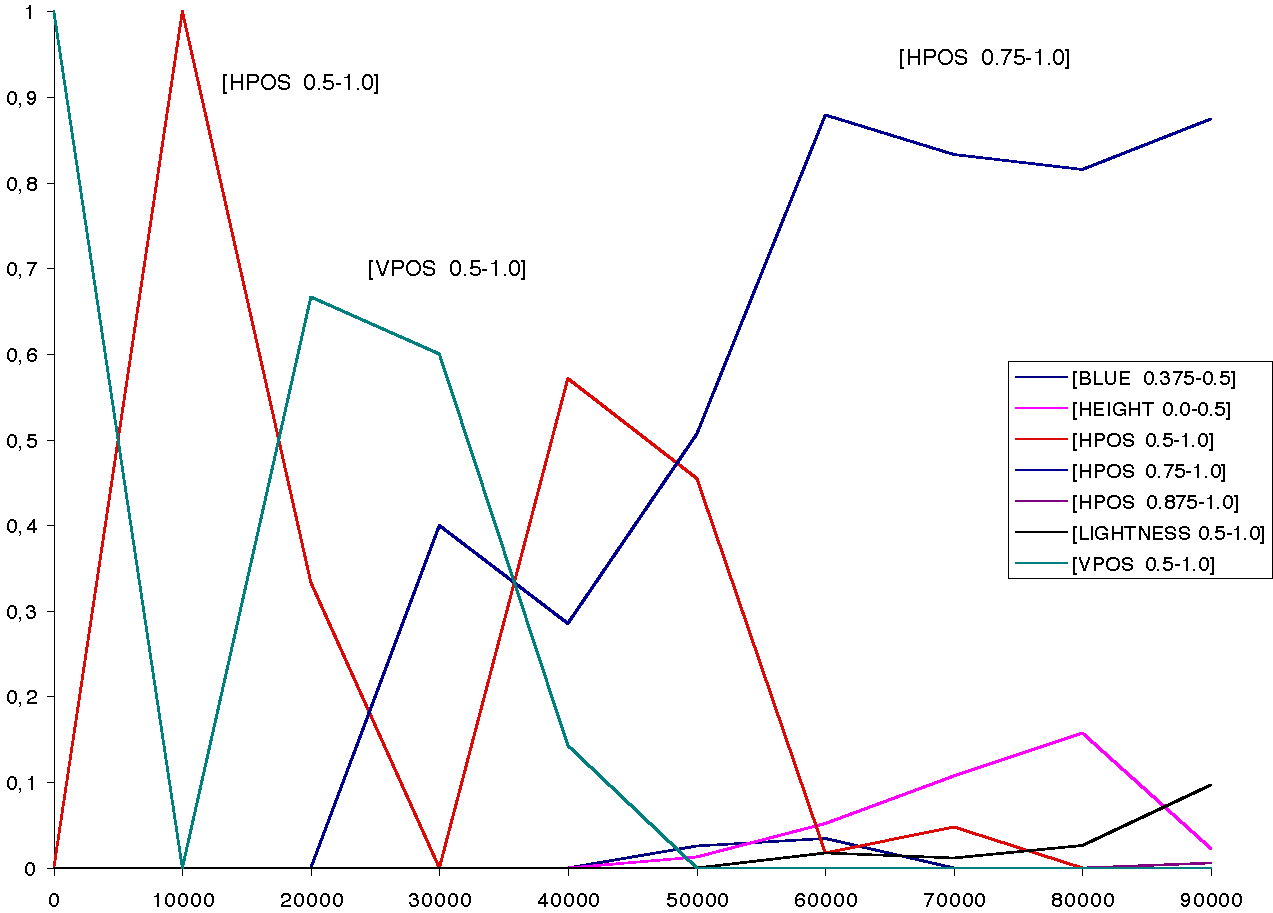
\includegraphics[width=.80\textwidth,height=6cm]{chap8/figures/droite}}
\caption{\label{fig:droite} 
Form-Meaning diagram: Different meanings associated with the word ``droite". The dominant meaning is 
in line with the human use of the word, namely horizontal position (HPOS) to the right of the image.}
\end{figure}

\figref{fig:bozopite} shows different meanings competing for the same word "bozopite". Dominant ones are 
a large area (AREA scaled between 0.5 and 1.0) or extended width (WIDTH scaled between 0.5 and 1.0). These two concepts
apparently could both be applied in many situations, but at some point new situations appeared that 
caused a symmetry breaking and AREA became dominant. 

\begin{figure}[htbp]
  \centerline{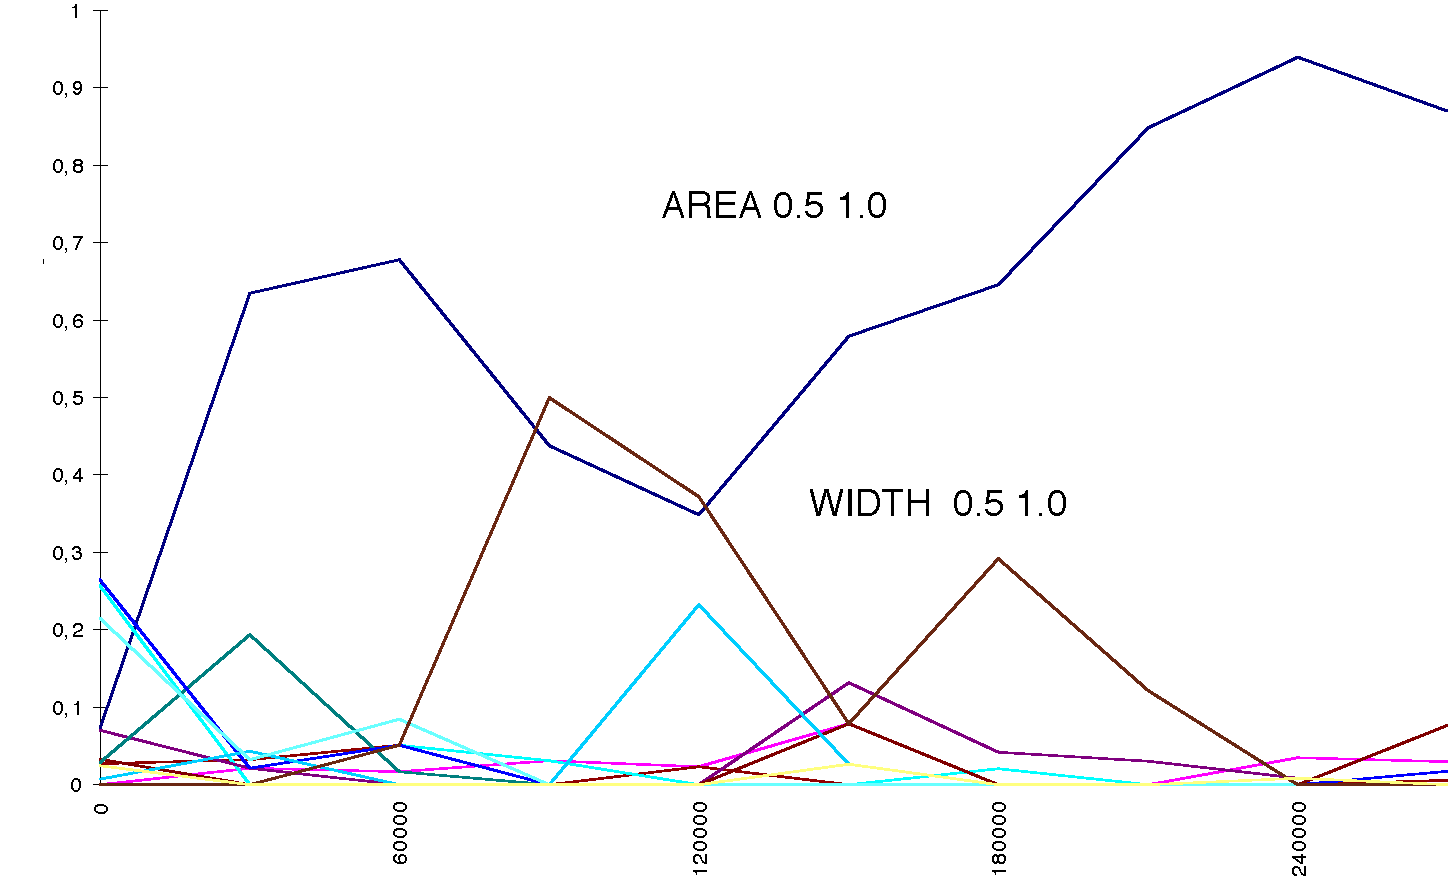
\includegraphics[width=.70\textwidth, height=6cm]{chap8/figures/bozopite}}
\caption{\label{fig:bozopite} 
Form-Meaning diagram: Different meanings associated with the word ``bozopite". 
}
\end{figure}

It was also possible that different meanings which were highly compatible were maintained in the population. 
An example is shown in the form-meaning diagram in \figref{fig:down}, which plots the average 
frequency of meanings for the word ``down". The meanings are all concepts on the vertical position channel 
VPOS, but they carve out smaller and smaller regions. 

\begin{figure}[htbp]
  \centerline{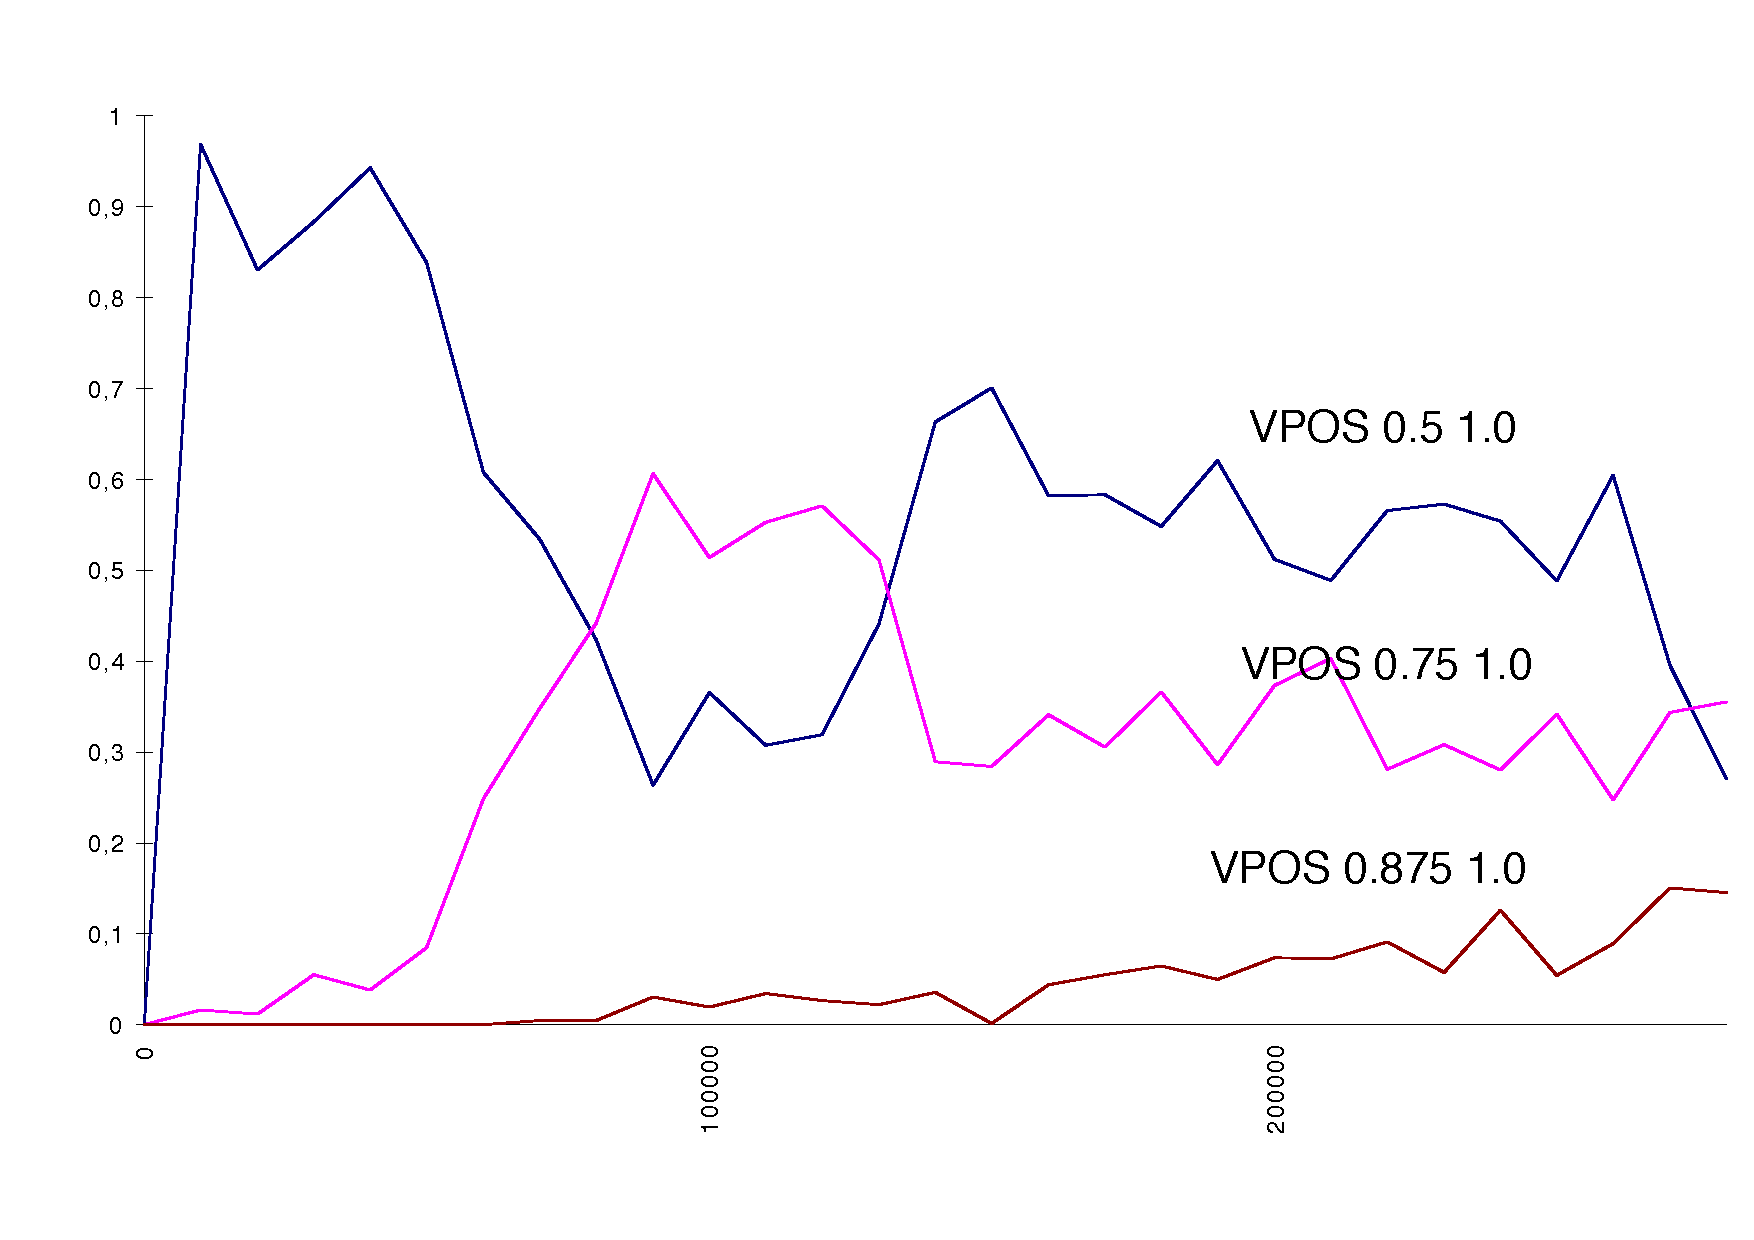
\includegraphics[width=.65\textwidth]{chap8/figures/down}}
\caption{\label{fig:down} 
Form-Meaning diagram: Different meanings associated with the word "down". There are in particular two meanings. 
one is a region on the red-channel and another one a region on the vertical position channel. 
}
\end{figure}

\section{Conclusions} 

The Talking Heads experiment was without doubt a success from many angles. The mechanisms for concept formation,
lexicon formation and alignment (as discussed in Part I of this book) all worked out the 
way it was expected, even in very difficult 'real world' conditions. The complex hardware could be maintained at the 
different physical sites and the general web infrastructure and agents teleportation mechanisms held up despite a 
significant scale-up. An enthusiastic user group formed and they actively created agents and sent 
them out on the network, often also teaching their agents human language words which then propagated
in the rest of the population. Users became very attached to their agents, upset when their agents could not get 
to the sites they had scheduled (because it took almost 1 minute for a complete language game and so other agents 
had to wait), and trying to figure out how and why they had learned certain words. 

Numerous talks were given and various papers published in scientific fora. There were also various talks within 
the art context\footnote{Examples are a 'gallery talk' as Salon 3 at the Elephant and Castle Centre
in London on 2 december 1998, organised by Hans Ulrich Obrist and Molly Nesbit, and a presentation together with 
Hans-Ulrich Obrist and Rem Koolhaas in Antwerp to launch the Laboratorium book on 3 october 2001.}
The experiment received wide coverage in 
the media thanks to its public exposure as part of a major exhibition. The Sued-Deutsche Zeitung called it 
`Angels with Internet wings'. All this lead to invitations to show the experiment
also in other venues, as discussed in the next chapter. 
Regretably, the challenge just to keep the experiment in the air with the available human resources
and the pressure for going on with new experiments prevented us from doing more adequate data gathering 
and analysis. Nevertheless some analyses appeared, particularly as carried out by Frederic Kaplan\cite{Kaplan:2001}. 

The field of complex systems science was at that time still in its infance and 
adequate tools for analysing language as a complex adaptive system were in the early stages of development. 
Nevertheles, various publications were 

The experiment ended with the following `tongue-in-cheek' post by Angus McIntyre on the Forum: \\

\begin{mail}
{\bfshape 1999-10-14 15:08:29 Angus McIntyre}\\
{\itshape Bad news and good news}\\

As the subject says, we have some bad news and some good news.

First, the bad news. The current run of the Talking Heads experiment will come to an end on the 5th of November. After that date, access to the system will be closed off, meaning that you won't be able to create, launch or inspect agents any more.

We realise that this will be a sad day for all of you who've participated so enthusiastically in the experiment. We will consider setting up self-help programs for anyone unable to cope with the pain of 'Talking Heads withdrawal'.

Now the good news. The Talking Heads *will* be back. We currently expect to launch an improved version of the system early in 2000, probably late in January. We shall use the intervening months to try to make our software faster and more stable. When the system returns, we should also have some new sites, both public and private. And we're thinking about trying to find ways to make the system more interesting (i.e. by giving you greater control over your agents and the way that they learn and interact with other agents).

If you'd like to comment on your experiences with the Talking Heads, or suggest ways that the system could be improved, this forum would be a good place to do that. I can't promise that we'll implement all your suggestions (we don't have very much time), but all your messages will certainly be read and considered.

In the meantime, on behalf of all the Talking Heads team, I'd just like to say 'thank you' to all of you for taking part and making the experiment a success.

     Angus McIntyre\\
     Agent Public Relations Officer
\end{mail}

Here is one commentary of a dedicated user: \\

\begin{mail}
{\bfshape 1999-10-27 18:52:04 Kampi}\\
{\itshape RE: Bad news and good news}

Are you crazy? Why do you do this at a time where winter with its long darkness is just ahead. Taking away 
from me the last beeings I can realy understand?
So, of course I'm very sad about the bad news. And I insist on a self-help program otherwise I don't know what will happen to me. I propose to create some kind of holiday-camp for my agents which I can run on my computer; for example with some beach scenery, quiet apartment with TV and pool and only a little bit of teaching abilities, so that they don't become totaly stupid although they will be able to recover from all these mad and debile cans in Paris, Brussels and Tokio; please implement the possibility that it's me who swiches off the light at night; then, and only then, I can be sure they have a good time until the restart.
But for serious: I hope very much that the Talking Heads will return as soon as possible. And I think you should inform those who are interested (me for example) by e-mail about the re-start.
Some wishes for the improved project: a better performance, especially for the lexicon. And much, much more information about the scientific background. How do the agents create their words? Are these guys on the Web realy part of the 'official'; experiment? Why did one of my agents suddenly create a three-part word (was there a bug in the software, how could it asume, that anyone would understand this, is it a syntactical genius and therefore its only natural that noone understands it or is it simply too stupid to understand the rules of the game? Is it the only agent who did this, why did it never try this again?... and so on). Anyway, more explanation for the 'future-heads'; about the experiment so that I understand why I should teach the agents. As far as I understood they were created to make sense (develop language) by their own.
Yes, I know, 'stop making sense';. It's their job, not mine.
Therefore at least a very big 'thank you; for having published the 'talking-heads'; on the net.

A very sad user

P.S.: Please send me the holidy camp including 2 single rooms and my agents caspar and Leyla as a zipped file by e-mail.
\end{mail}



